\documentclass[../ap_2016.tex]{subfiles}

\graphicspath{{./image/}}

\begin{document}

\setcounter{chapter}{2}
\chapter{複素解析:調和関数}
\section{}
\subsection{}
\begin{equation}\begin{aligned}[b]
    w &= \sin(x+iy) = \sin(x)\cos(iy)+\cos(x)\sin(iy)\\
    u +iv &= \sin(x)\cosh(y)+i\cos(x)\sinh(y)
\end{aligned}\end{equation}

\subsection{}
\(x=c\)を[1-1]に代入すると
\begin{equation}\begin{aligned}[b]
    u &= \sin(c)\cosh(y), & v &= \cos(c)\sinh(y)
\end{aligned}\end{equation}
となるので、
\begin{equation}\begin{aligned}[b]
    1 &= \cosh^2(y)-\sinh^2(y)=\qty(\frac{u}{\sin(c)})^2-\qty(\frac{v}{\cos(c)})
\end{aligned}\end{equation}
これをプロットすると図3.1のようになる。

これよ領域\(D_1\)は、\(w\)平面上では\(u\geq0,v\geq0\)に移されるのがわかる

\begin{figure}[h]
    \centering
    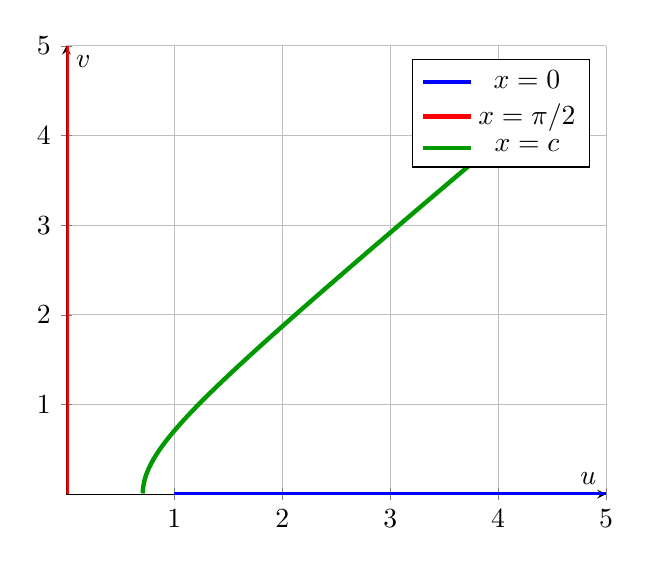
\begin{tikzpicture}
        % --- 定数の定義 (角度は度数法) ---
        \def\a{45} % cos(t) > 0 となるように設定 (例: -90 < t < 90)

        \begin{axis}[
            xlabel={$u$},
            ylabel={$v$},
            grid=major,
            axis lines=middle, % 軸を中央に配置
            xmin=0, % 制約 x > 0
            ymin=0, % 制約 y > 0
            xmax=5,
            ymax=5,
            legend pos=north east,
            % 定数の値をプロット内に表示
        ]
            \addplot[
                domain=1:\pgfkeysvalueof{/pgfplots/xmax}, % x=1からグラフの右端まで
                samples=2, % 直線なのでサンプルは2点でOK
                color=blue,
                ultra thick % かなり太い線
            ]{0};
            \addlegendentry{$x=0$}

            \addplot[
                color=red,
                ultra thick
            ] coordinates {(0, \pgfkeysvalueof{/pgfplots/ymin}) (0, \pgfkeysvalueof{/pgfplots/ymax})};
            \addlegendentry{$x=\pi/2$}

            \addplot[
                domain=0.01:2.5,
                samples=100, % 滑らかさ
                color=green!60!black,
                ultra thick
            ]
            ({sin(\a)*cosh(x)}, {cos(\a)*sinh(x)});
            \addlegendentry{$x=c$}

        \end{axis}
    \end{tikzpicture}
    \caption{[1-2]の回答}
\end{figure}

\section{}
\subsection{}
Cauchy-Riemann の関係式より
\begin{equation}\begin{aligned}[b]
    \pdv{u}{x}&=\pdv{v}{y},& \pdv{u}{y}=-\pdv{u}{x}
\end{aligned}\end{equation}
これらの両辺を\(x\)微分、\(y\)微分をして
\begin{equation}\begin{aligned}[b]
    \pdv[2]{u}{x} &= \pdv{v}{x}{y}, & \pdv{u}{x}{y}=-\pdv[2]{v}{x}\\
    \pdv{u}{x}{y} &= \pdv[2]{v}{y}, & \pdv[2]{u}{y}=-\pdv{v}{x}{y}
\end{aligned}\end{equation}
これらを組み合わせると
\begin{equation}\begin{aligned}[b]
    \pdv[2]{u}{x}+\pdv[2]{u}{y}&=0\\
    \pdv[2]{v}{x}+\pdv[2]{v}{y}&=0
\end{aligned}\end{equation}
となり、示せた。

\subsection{}
\begin{equation}\begin{aligned}[b]
    \pdv[2]{H}{x}+\pdv[2]{H}{y}
    &= \pdv{x}\qty(\pdv{u}{x}\pdv{h}{x}+\pdv{v}{x}\pdv{h}{v})+\pdv{y}\qty(\pdv{u}{y}\pdv{h}{u}+\pdv{v}{y}\pdv{h}{v})\\
    &= \pdv[2]{u}{x}\pdv{h}{u}+\qty(\pdv{u}{x})^2\pdv[2]{h}{u}+\pdv[2]{v}{x}\pdv{h}{v}+\qty(\pdv{v}{x})^2\pdv[2]{h}{v}\\
    &\qquad +\pdv[2]{u}{y}\pdv{h}{u}+\qty(\pdv{u}{y})^2\pdv[2]{h}{u}+\pdv[2]{v}{y}\pdv{h}{v}+\qty(\pdv{v}{y})^2\pdv[2]{h}{v}\\
    &=\qty(\pdv[2]{u}{x}+\pdv[2]{u}{y})\pdv{h}{u}+\qty(\pdv[2]{y}{x}+\pdv[2]{y}{y})\pdv{h}{y}\\
    &\qquad +\qty{\qty(\pdv{u}{x})^2+\qty(\pdv{u}{y})^2}\pdv[2]{h}{u} + \qty{\qty(\pdv{v}{x})^2+\qty(\pdv{v}{y})^2}\pdv[2]{h}{v}\\
    &=\qty{\pdv{u}{x}\pdv{u}{y}-\pdv{u}{y}\pdv{v}{x}+\pdv{u}{y}\pdv{v}{x}-\pdv{u}{x}\pdv{v}{y}}\pdv[2]{h}{u}\\
    &=0
\end{aligned}\end{equation}
より、\(H(x,y)\)は調和関数

\section{}
\subsection{}
\(z=\arcsin(w)\)より\(0\leq x \leq \frac{\pi}{2},y\geq 0\).

(1)の条件のうち
\(u=0\)は
\begin{equation}\begin{aligned}[b]
    0 &= \sin(x)\cosh(y) & \rightarrow x = 0
\end{aligned}\end{equation}
\(v\geq 0\)は\(\cos(x)\sinh(y)\geq 0\)となるため自動的に満たす。
よって
\begin{equation}\begin{aligned}[b]
    H(0,y)=0
\end{aligned}\end{equation}

(2)の条件のうち、
\(v=0\)は
\begin{equation}\begin{aligned}[b]
    0 &= \cos(x)\sinh(y) & \rightarrow x=\frac{\pi}{2}\quad\text{or}\quad y = 0
\end{aligned}\end{equation}
\(u\geq 1\)は
\begin{equation}\begin{aligned}[b]
    \sin(x)\cosh(y)\geq 1
\end{aligned}\end{equation}
\(x=\frac{\pi}{2}\)のときは\(y\geq0\), \(y=0\)のときは\(x=\frac{\pi}{2}\)より
いずれにせよ\(x=\frac{\pi}{2}\)が条件となる。
よって
\begin{equation}\begin{aligned}[b]
    H\qty(\frac{\pi}{2},y)&=1
\end{aligned}\end{equation}

(3)の条件のうち、
\(v=0\)は
\begin{equation}\begin{aligned}[b]
    0 &= \cos(x)\sinh(y) & \rightarrow x=\frac{\pi}{2}\quad\text{or}\quad y = 0
\end{aligned}\end{equation}
\(0\leq u\leq 1\)の条件が\(x=\frac{\pi}{2}\)のときは
\begin{equation}\begin{aligned}[b]
    0&\leq\sin(x)\cosh(y)\leq 1\\
     0&\leq\cosh(y)\leq 1\\
    y&= 0
\end{aligned}\end{equation}
\(y=0\)のときには
\begin{equation}\begin{aligned}[b]
    0&\leq\sin(x)\leq 1
\end{aligned}\end{equation}
よってヤコビアンを計算して
\begin{equation}\begin{aligned}[b]
    0 &= \pdv{x}{v}\pdv{H}{x}+\pdv{y}{v}\pdv{H}{y}\\
    &= -\sin(x)\sinh(y)\pdv{H}{x}+\cos(x)\cosh(y)\pdv{H}{y}
\end{aligned}\end{equation}
\(x=\frac{\pi}{2},y=0\)のときは自動的に満たす。
よって\(y=0\)のときを考えて、
\begin{equation}\begin{aligned}[b]
    \pdv{H}{y}(x,0)=0
\end{aligned}\end{equation}

まとめると
\begin{equation}\begin{aligned}[b]
    H(0,y) &= 0\\
    H\qty(\frac{\pi}{2},y) &= 0\\
    \pdv{H}{y}(x,0) &=0
\end{aligned}\end{equation}

\subsection{}


\end{document}
